\section{Nurul Izza Hamka | 1174062}
\subsection{Teori}
\begin{enumerate}

\item Apa itu Binary Classification dilengkapi Ilustrasi Buatan sendiri
Binary Classification adalah  mengklasifikasikan sebuah elemen-elemen dari suatu himpunan yang di masukkan kedalam dua kelompok dengan memprediksi  kelompok mana yang masing-masing dimiliki berdasarkan aturan klasifikasi. Konteks yang memerlukan keputusan apakah suatu item memiliki sifat kualitatif atau tidak, beberapa karakteristik tertentu, atau beberapa klasifikasi biner khas

\begin{figure}[H]
	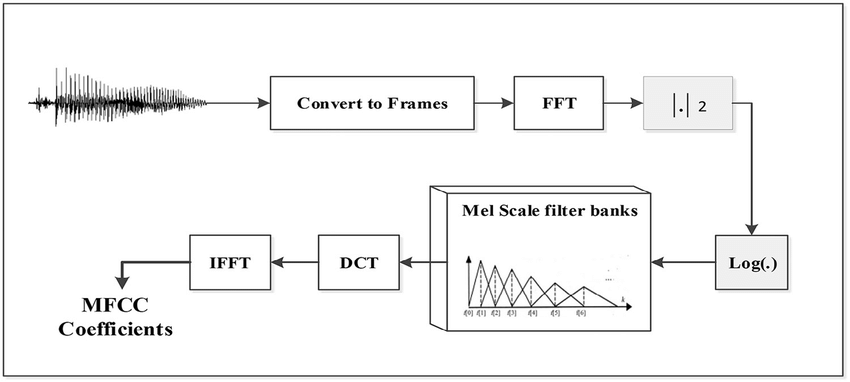
\includegraphics[width=4cm]{figures/1174062/Teori/no1.PNG }
	\centering
	\caption{Gambar Binary Classification }
\end{figure}

\item Apa itu supervised Learning, Unsupervised Learning, dan Clustering dengan ilustrasi sendiri

Pengertian dalam konteks AI, supervised learning adalah sistem dimana sebuah input dan output data yang kita inginkan sudah tersedia. Input dan output data ini diberi label untuk klasifikasi dasar pembelajaran untuk pemrosesan data yang akan datang. Supervised learing ini menyediakan algoritma untuk pembelajaran dengan jumlah diketahui untuk mendukung sebuah penilaian yang akan datang.\\

\begin{figure}[H]
	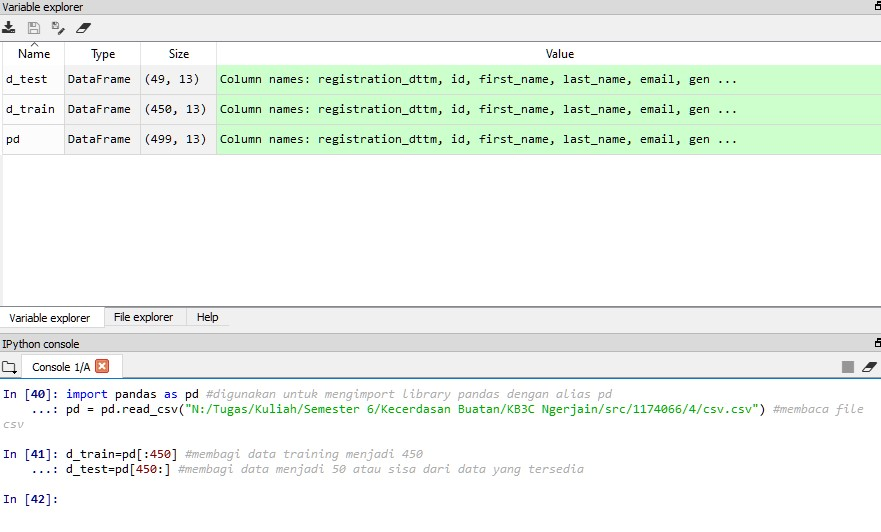
\includegraphics[width=4cm]{figures/1174062/Teori/no2.PNG }
	\centering
	\caption{Gambar Supervised Learning }
\end{figure}

Unsupervised Learning tidak memiliki data latih, sehingga dari data yang telah ada kita kelompokkan menjadi dua ataupun tiga bagian dst. Unsupervised learning ini merupakan pelatihgan algoritma kecerdasan buatan menggunakan infomasi yang tidak diklasifikasikan atau diberi label dan memungkinkan algoritma untuk bertindak atas informasi tersebut tanpa bimbingan.\\

\begin{figure}[H]
	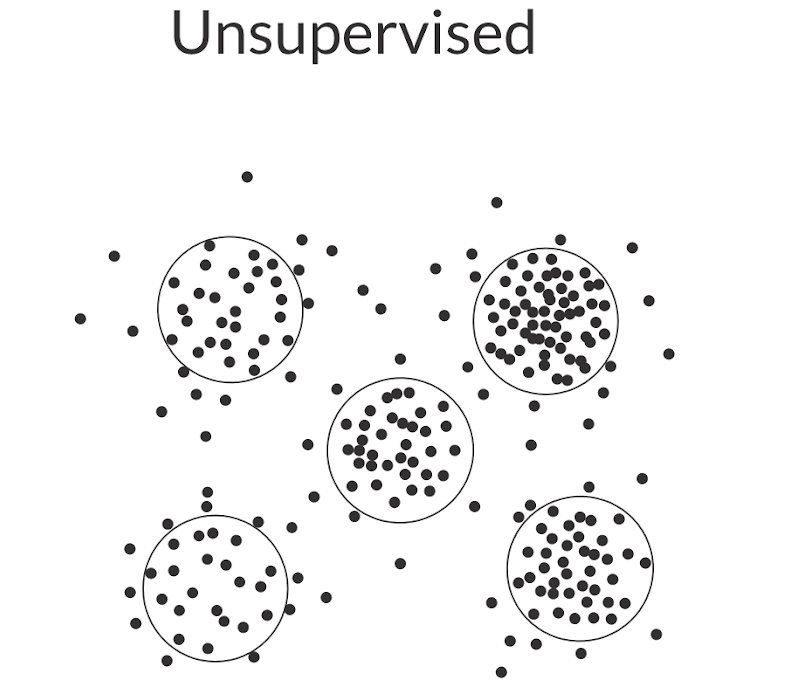
\includegraphics[width=4cm]{figures/1174062/Teori/Unsupervised.PNG }
	\centering
	\caption{Gambar Unsupervised Learning }
\end{figure}

Clustering adalah pengelompokan objek dengan sedemikian rupa sehingga objek berada dalam kelompok yang sama (disebut klister) lebih mirip satu sama lain dibandingkan kelompok lain. 

\begin{figure}[H]
	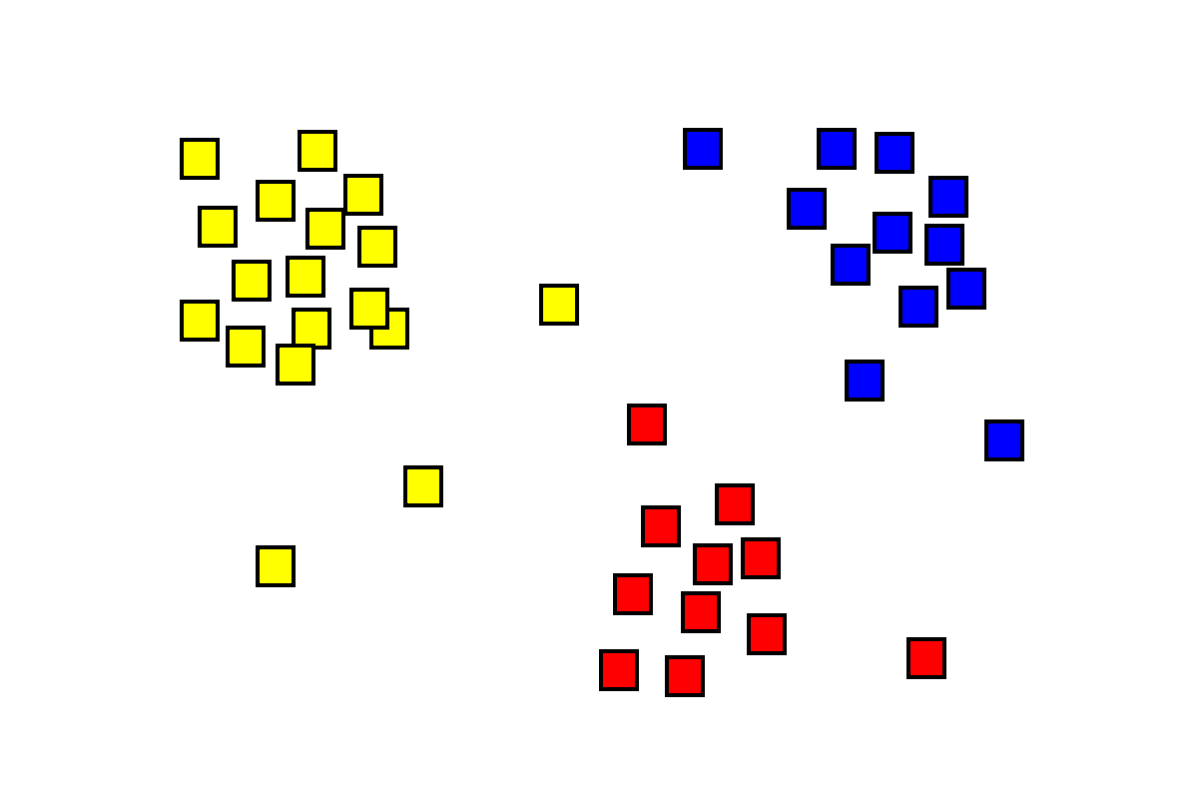
\includegraphics[width=4cm]{figures/1174062/Teori/Clustering.PNG }
	\centering
	\caption{Gambar Clustering }
\end{figure}

\item Apa itu evaluasi dan akurasi dari buku dan disertai contoh dengan gambar sendiri.

Evaluasi adalah bagaimana kita dapat melakukan evaluasi tentang seberapa baik model bekerja dengan mengukur tingkat akurasinya.\\
 
Akurasi ini didefinisikan sebagai sebuah persentase kasus yang diklasifikasikan dengan benar. Analisis dapat dilakukan menggunakan sebuah matriks kebingungan apabila model yang dibuat terdapat kesalaha atau tingkat kebingungannya.

\item Bagaimana cara membuat dan membaca cunfusion matrix, buat cunfusion matrix buatan sendiri

Confusion matrix adalah untuk memberikan informasi sebuah oerbandingan hasil klasifikasi yang di lakukan oleh sebuah sistem atau model dengan hasil klasifikasi yang nyata.\\
Cara membuat dan membaca cunfosion matrix:\\
1. Tentukan pokok permasalahan dan atributanya, misal gaji dan listik.\\
2. Buat pohon keputusan.\\
3. Lalu data testingnya.\\
4. Lalu mencari nilai a, b, c, dan d.\\
5. Selanjutnya mencari nilai recall, precision, accuracy, serta dan error rate.

\begin{figure}[H]
	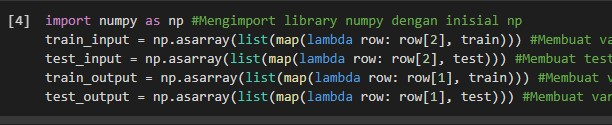
\includegraphics[width=4cm]{figures/1174062/Teori/no4.PNG }
	\centering
	\caption{Gambar Cunfusion Matrix }
\end{figure}

\item Bagaimana K-fold cross validation bekerja, disertai gambar ilustrasi contoh buatan sendiri

K-fold cross validation adalah salah satu metode yang mengevaluasi kinerja classfier, metode ini dapat kita gunakan jika jumlah data terbatas atau jumlah instance tidak banyak.\\

Cara kerja K-fold Cross validation adalah :\\
1. Total instance dibagi menjadi N bagian.\\
2. Fold ke 1 adalah bagian pertama menjadi data uji (testing data) dan sisanya menjadi training data.\\
3. Fold yang kedua adalah ketika ke 2 menjadi data uji dan sisanya menjadi data latih\\
4. Hitung akurasi berdasarkan porsi data tersebut\\
5. Begitupun dengan selanjutnya hingga mencapai fold ke-K, dan hitung rata-rata akurasi daari K buah akurasi tersebut.\\

\begin{figure}[H]
	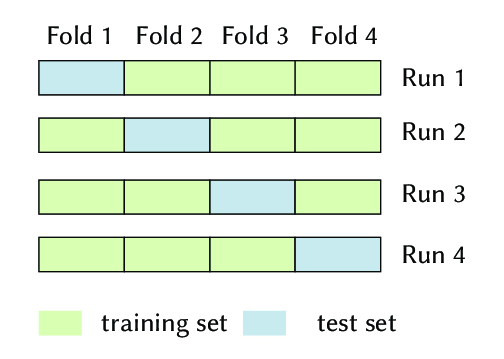
\includegraphics[width=4cm]{figures/1174062/Teori/K-fold.PNG }
	\centering
	\caption{Gambar K-Fold Cross Validation }
\end{figure}

\item Apa itu desicion tree, buat gambar ilustrasi contoh buatan sendiri

Decision tree adalah sebuah metode pembelajaran non-parametik yang digunakan untuk klasifikasi dan juga regrasi. Tujuannya adalah untuk membuat sebuah model yang dapat memprediksi sebuah nilai variable target dengan memahami aturan sederhana dari fitur data.

\begin{figure}[H]
	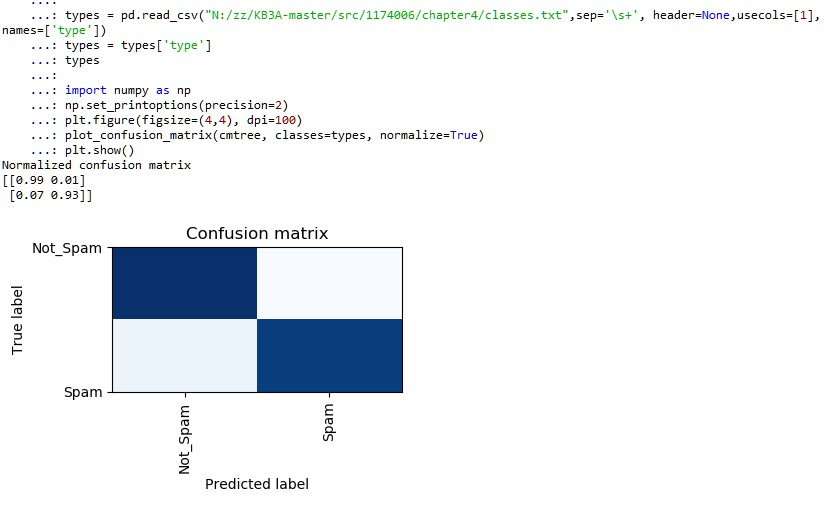
\includegraphics[width=4cm]{figures/1174062/Teori/no6.PNG }
	\centering
	\caption{Gambar Decision Tree }
\end{figure}

\item Apa itu Information gain dan entropi, gambar ilustrasi contoh buatan sendiri.

Information gain adalah penurunan entropi setelag dataset dibagi pada sebuah atribut. Dalam membangun decision tree semua tentang menemukan atribut yang mengembalikan prolehan informasi tertinggi.\\

\begin{figure}[H]
	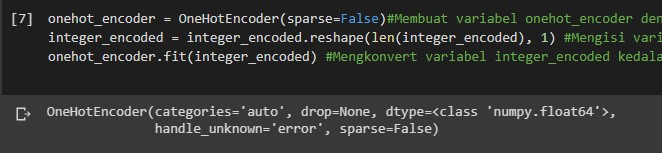
\includegraphics[width=4cm]{figures/1174062/Teori/no7.PNG }
	\centering
	\caption{Gambar Information Gain }
\end{figure}

Entropi merupakan ukuran keacakan dalam sebuah informasi yang sedang diproses. Semakin tinggi sebuah entropi  maka semakin sulit menarik sebuah kesimpulan dari informasi tersebut.

\begin{figure}[H]
	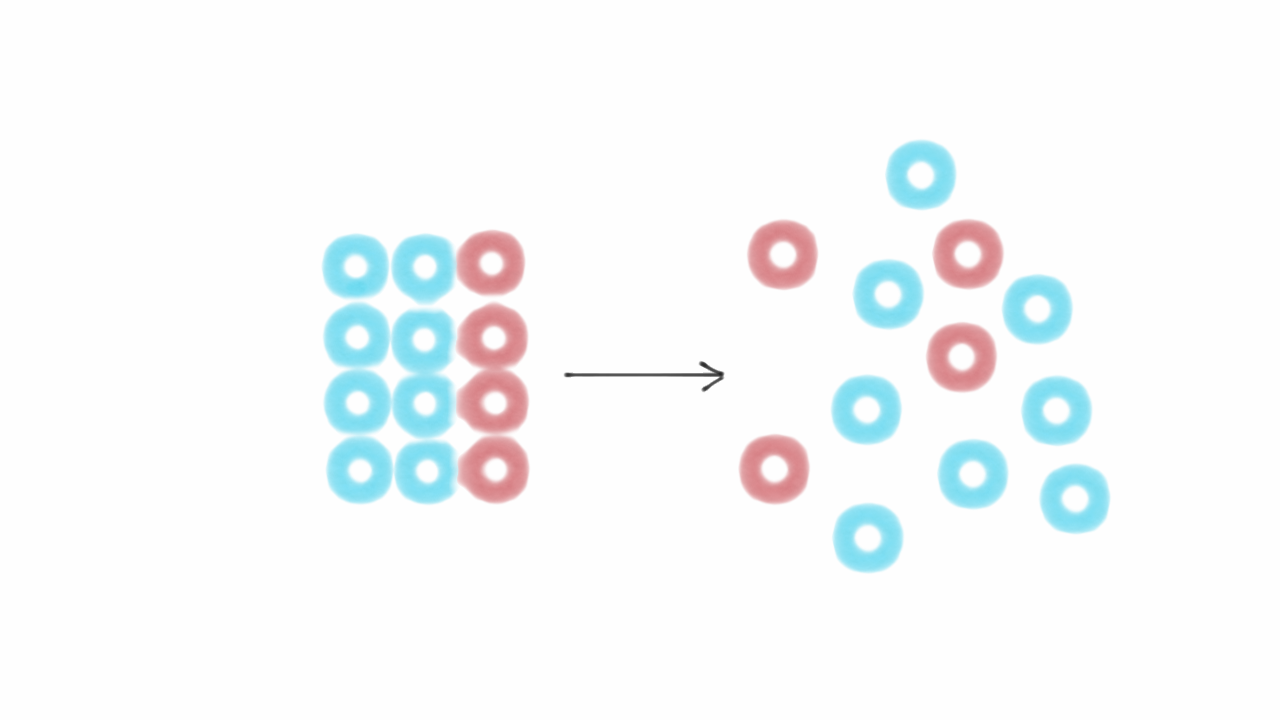
\includegraphics[width=4cm]{figures/1174062/Teori/Entropy.PNG }
	\centering
	\caption{Gambar Binary Classification }
\end{figure}

\subsection{Scikit-learn}
\begin{enumerate}
	\item Nomor 1
	\hfill\break
	\lstinputlisting[firstline=8, lastline=13]{src/1174062/2/1174062.py}
	
\begin{figure}[H]
	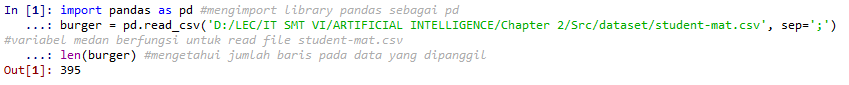
\includegraphics[width=4cm]{figures/1174062/ScikitLearn/Nomor 1.PNG }
	\centering
	\caption{Gambar Hasil No 1 }
\end{figure}
	
\item Nomor 2
	\hfill\break
	\lstinputlisting[firstline=15, lastline=20]{src/1174062/2/1174062.py}
	
\begin{figure}[H]
	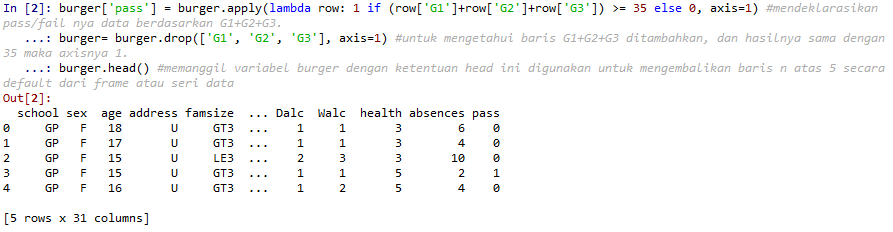
\includegraphics[width=4cm]{figures/1174062/ScikitLearn/Nomor 2.PNG }
	\centering
	\caption{Gambar Hasil No 2 }
\end{figure}
	
\item Nomor 3
	\hfill\break
	\lstinputlisting[firstline=22, lastline=28]{src/1174062/2/1174062.py}
	
\begin{figure}[H]
	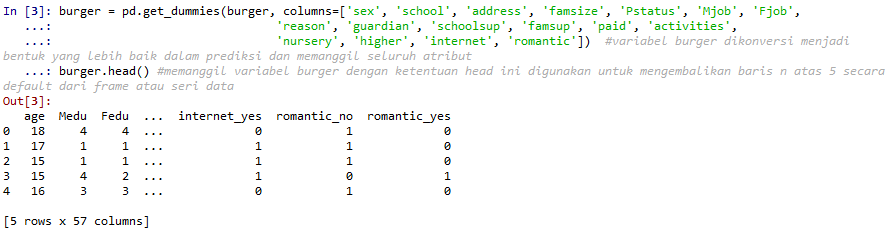
\includegraphics[width=4cm]{figures/1174062/ScikitLearn/Nomor 3.PNG }
	\centering
	\caption{Gambar Hasil No 3 }
\end{figure}

\item Nomor 4
	\hfill\break
	\lstinputlisting[firstline=30, lastline=49]{src/1174062/2/1174062.py}
	
\begin{figure}[H]
	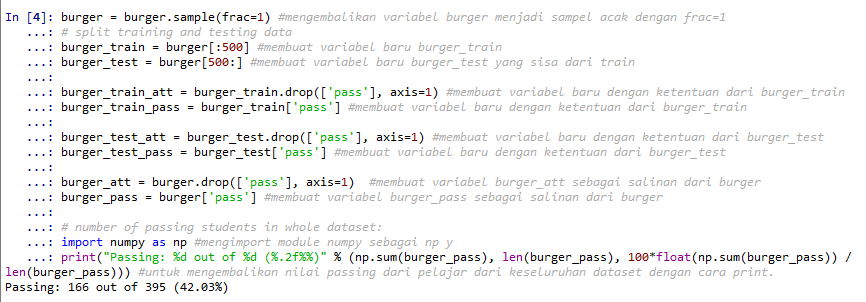
\includegraphics[width=4cm]{figures/1174062/ScikitLearn/Nomor 4.PNG }
	\centering
	\caption{Gambar Hasil No 4 }
\end{figure}

\item Nomor 5
	\hfill\break
	\lstinputlisting[firstline=51, lastline=56]{src/1174062/2/1174062.py}
	
\begin{figure}[H]
	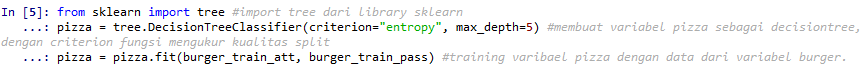
\includegraphics[width=4cm]{figures/1174062/ScikitLearn/Nomor 5.PNG }
	\centering
	\caption{Gambar Hasil No 5 }
\end{figure}
	
\item Nomor 6
	\hfill\break
	\lstinputlisting[firstline=58, lastline=68]{src/1174062/2/1174062.py}
	
\begin{figure}[H]
	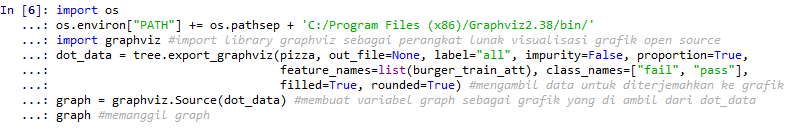
\includegraphics[width=4cm]{figures/1174062/ScikitLearn/Nomor 6.PNG }
	\centering
	\caption{Gambar Hasil No 6 }
\end{figure}
	
\begin{figure}[H]
	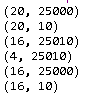
\includegraphics[width=4cm]{figures/1174062/ScikitLearn/6.PNG }
	\centering
	\caption{Gambar Hasil No 6 }
\end{figure}
	
\item Nomor 7
	\hfill\break
	\lstinputlisting[firstline=70, lastline=75]{src/1174062/2/1174062.py}
	
\begin{figure}[H]
	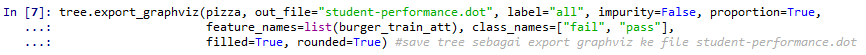
\includegraphics[width=4cm]{figures/1174062/ScikitLearn/Nomor 7.PNG }
	\centering
	\caption{Gambar Hasil No 7 }
\end{figure}
	
\item Nomor 8
	\hfill\break
	\lstinputlisting[firstline=77, lastline=80]{src/1174062/2/1174062.py}
	
\begin{figure}[H]
	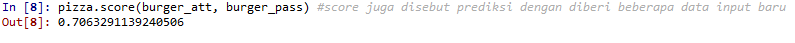
\includegraphics[width=4cm]{figures/1174062/ScikitLearn/Nomor 8.PNG }
	\centering
	\caption{Gambar Hasil No 8 }
\end{figure}
	
\item Nomor 9
	\hfill\break
	\lstinputlisting[firstline=82, lastline=87]{src/1174062/2/1174062.py}
	
\begin{figure}[H]
	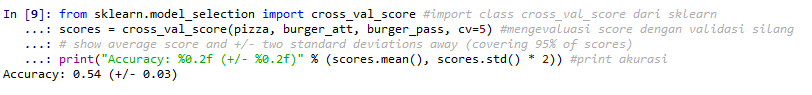
\includegraphics[width=4cm]{figures/1174062/ScikitLearn/Nomor 9.PNG }
	\centering
	\caption{Gambar Hasil No 9 }
\end{figure}
	
\item Nomor 10
	\hfill\break
	\lstinputlisting[firstline=89, lastline=95]{src/1174062/2/1174062.py}
	
\begin{figure}[H]
	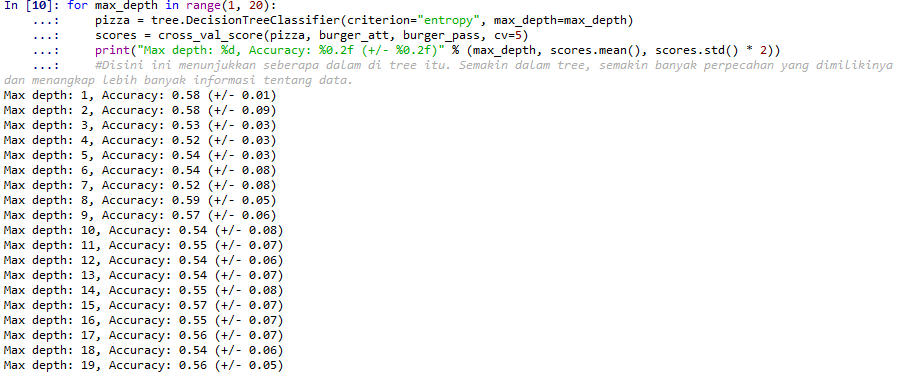
\includegraphics[width=4cm]{figures/1174062/ScikitLearn/Nomor 10.PNG }
	\centering
	\caption{Gambar Hasil No 10 }
\end{figure}

\item Nomor 11
	\hfill\break
	\lstinputlisting[firstline=97, lastline=109]{src/1174062/2/1174062.py}
	
\begin{figure}[H]
	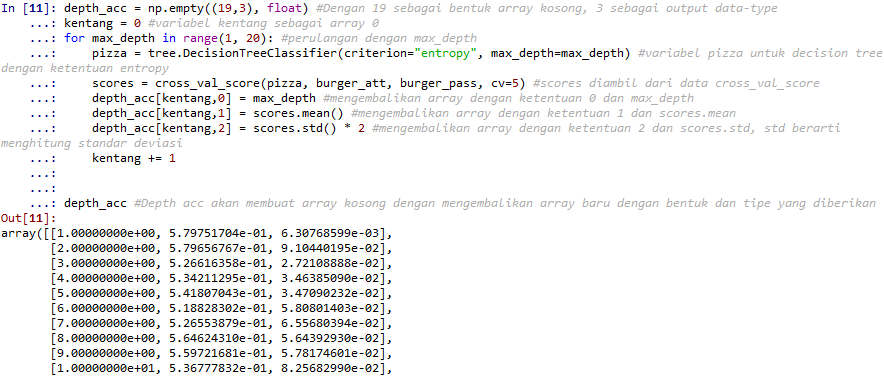
\includegraphics[width=4cm]{figures/1174062/ScikitLearn/Nomor 11.PNG }
	\centering
	\caption{Gambar Hasil No 11 }
\end{figure}	

\item Nomor 12
	\hfill\break
	\lstinputlisting[firstline=111, lastline=116]{src/1174062/2/1174062.py}
	
\begin{figure}[H]
	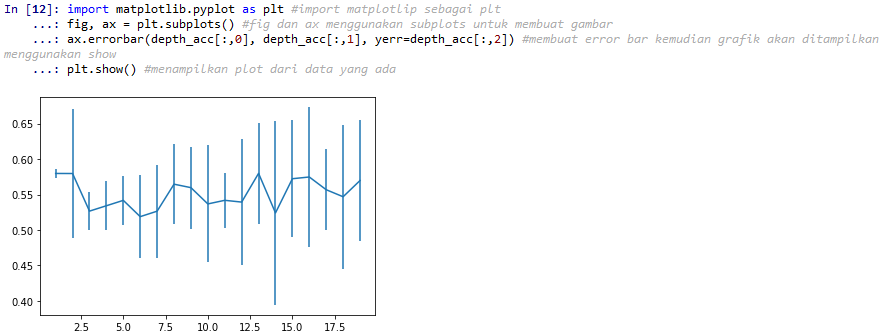
\includegraphics[width=4cm]{figures/1174062/ScikitLearn/Nomor 12.PNG }
	\centering
	\caption{Gambar Hasil No 12 }
\end{figure}
	
\begin{figure}[H]
	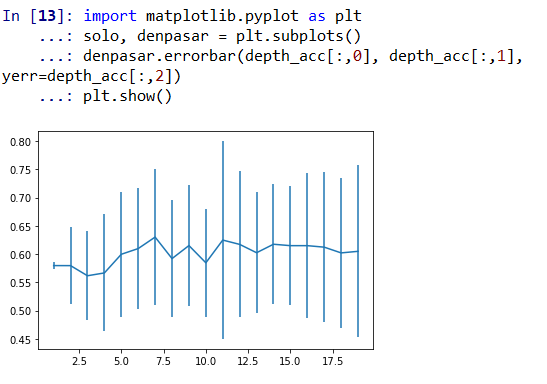
\includegraphics[width=4cm]{figures/1174062/ScikitLearn/12.PNG }
	\centering
	\caption{Gambar Hasil No 12 }
\end{figure}
	
\end{enumerate}

\subsection{Penanganan error}

\item Hasil Screenshoot Error
\begin{figure}[H]
	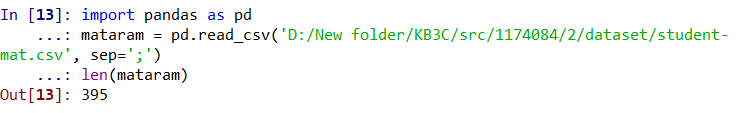
\includegraphics[width=4cm]{figures/1174062/Error/1.PNG }
	\centering
	\caption{Gambar Module Not Found Error }
\end{figure}
\item Cara penanganannya adalah dengan memperbaiki penulisanya yang salah dalam penulisan kode atau melakukan penginstallan package atau modul yang belum terinstal.\\

\begin{figure}[H]
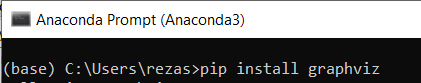
\includegraphics[width=4cm]{figures/1174062/Error/2.PNG }
	\centering
	\caption{Gambar Error Bagian 2 }
\end{figure}
\item Cara penangananya adalah memperbaiki directory file. Dengan menyesuaikan tempat penyimpanan di laptop.\\

\begin{figure}[H]
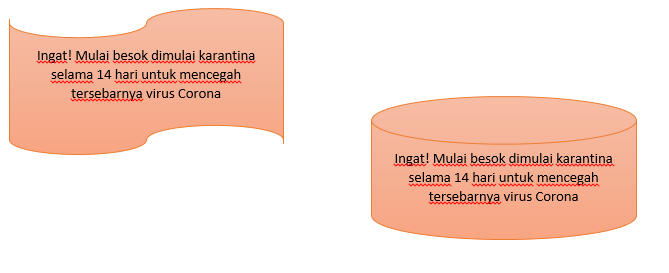
\includegraphics[width=4cm]{figures/1174062/Error/3.PNG }
	\centering
	\caption{Gambar Error Bagian 3 }
\end{figure}
\item Cara penanganannya lakukan penginstallan graphviz di windows dan menambahkan directory diatas pada kode program

\subsection{Bukti Tidak Plagiat}

\item Bukti Tidak Melakukan Plagiat
\begin{figure}[H]
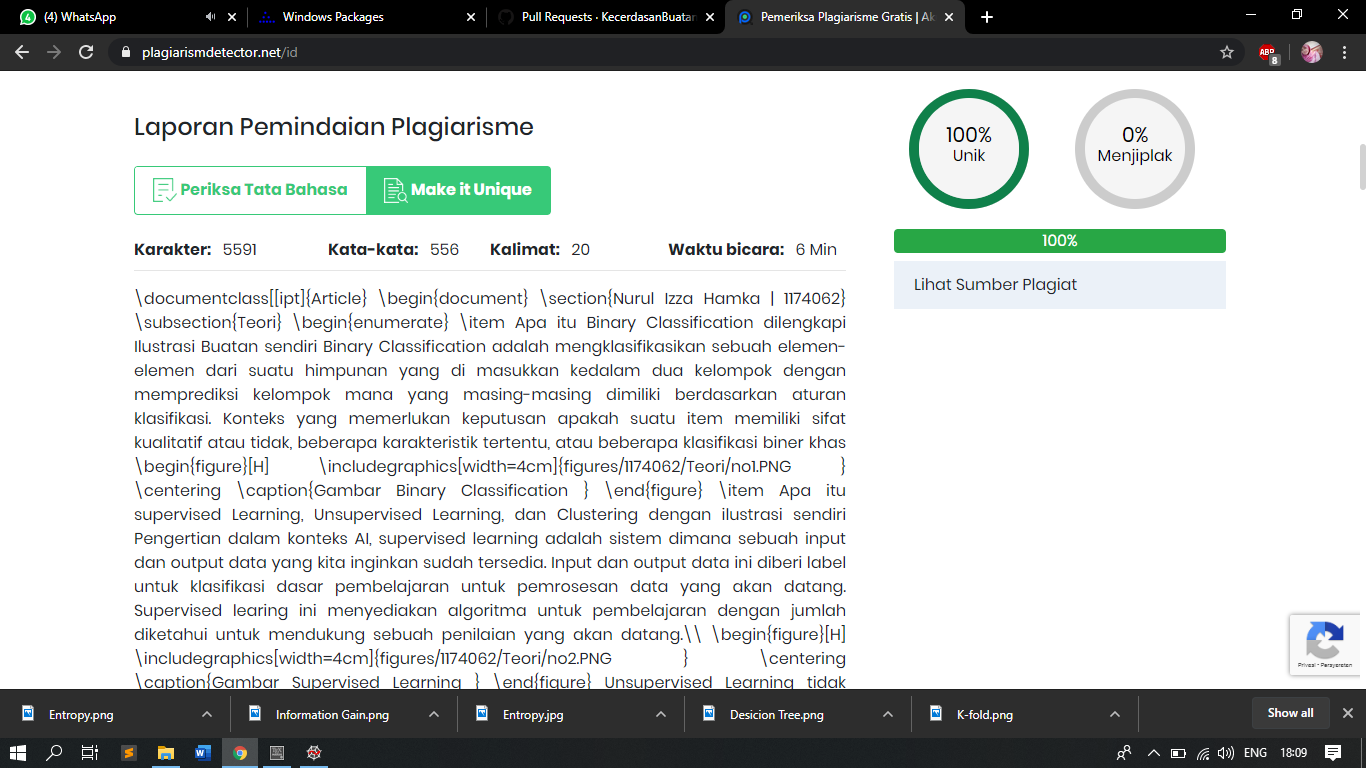
\includegraphics[width=4cm]{figures/1174062/Plagiat/Tidakplagiat.PNG}
	\centering
	\caption{Bukti Tidak Plagiat }
\end{figure}

\subsection{Link Youtube}

\end{enumerate}
